\documentclass[11pt, oneside]{article}   	% use "amsart" instead of "article" for AMSLaTeX format
\usepackage{geometry}                		% See geometry.pdf to learn the layout options. There are lots.
\geometry{letterpaper}                   		% ... or a4paper or a5paper or ... 
\usepackage{graphicx}				% Use pdf, png, jpg, or eps§ with pdflatex; use eps in DVI mode
								% TeX will automatically convert eps --> pdf in pdflatex		
\usepackage{amssymb}
 \usepackage{amsmath}
\usepackage[]{algorithm2e} 			% for the pseudocode

\date{}							% Activate to display a given date or no date
\parindent 0in
\parskip 6pt


 
\begin{document}

\title{\bf Solving partial differential equations in two dimensions using finite differences }

\maketitle
 
%\section*{Learning Goals}
%In this lecture you will learn about:
%\begin{itemize}
%\item  
%\end{itemize}

%------------------------------------------------------------------------------------------
\section*{Review of finite differences in 1D}
%------------------------------------------------------------------------------------------

Earlier in this course when we looked at transient groundwater modeling, you were introduced to the one dimension diffusion equation, which has the basic form:
\begin{eqnarray}
 	\frac{\partial u}{\partial t} =   \frac{\partial^2 u}{\partial x^2}  
\end{eqnarray} 
where here we omit the material property coefficient terms to keep things simple.  You also learned how to approximate the partial derivatives in this expression using finite differences computed between discrete samples of $u$. The first order partial derivative has the forward finite difference approximation:
\begin{eqnarray}
	\frac{\partial u(t_i)}{\partial t}  \approx \frac{u(t_{i+1}) - u(t_i)}{\Delta t} ,
\label{FOFD}
\end{eqnarray}
where  $\Delta t$ is   $t_{i+1} - t_i$. You also saw the second order partial derivative  has the central finite difference approximation:
\begin{eqnarray}
	\frac{\partial^2 u(x_i)}{\partial x^2}  & \approx& \frac{u(x_{i+1}) - 2 u(x_i) + u(x_{i-1})  }{\Delta x^2} ,
\label{SOFD}
\end{eqnarray}
where  $\Delta x$ is the grid spacing in $x$. We also simplified the notation by using $u_i = u(x_i)$, giving:
\begin{eqnarray}
	\frac{\partial^2 u_i}{\partial x^2}  & \approx& \frac{u_{i+1} - 2 u_i + u_{i-1}  }{\Delta x^2}  
\label{SOFD2}
\end{eqnarray}
 
%------------------------------------------------------------------------------------------
\section*{Two dimensional Partial Differential Equations}
%------------------------------------------------------------------------------------------
We will expand the finite difference method to two dimension so we can model the behavior of a function $u$ in both the $x$ and $y$ directions: $u = u(x,y)$.  Here are three commonly encountered two dimension partial differential equations:
\begin{eqnarray}
	\frac{\partial^2 u}{\partial x^2}   + \frac{\partial^2 u}{\partial y^2}&=&   0 \;\;\;\;\;\;\;\;\;\; \textrm{Laplace's equation} \\
 	  \frac{\partial^2 u}{\partial x^2}   + \frac{\partial^2 u}{\partial y^2}&=&  \frac{\partial u}{\partial t} \;\;\; \;\;\;\; \textrm{Diffusion equation} \\
	   \frac{\partial^2 u}{\partial x^2}   + \frac{\partial^2 u}{\partial y^2}&=&  \frac{\partial^2 u}{\partial t^2}  \;\;\;\;\;\; \textrm{Wave equation} 
\end{eqnarray}
 Notice how these equations are all nearly the same. The differences are in the time dependent terms on the right hand side. Laplace's equation has no time dependence, and can be thought of as the steady state solution to either the diffusion of wave equations. The diffusion equation has a first order time derivative while the wave equation has a second order time derivative.
 
 Here these equations are presented in their generic coefficient-free form. When applying them to real problems, we will have to include terms that account for the material properties of the problem (for example, like the hydraulic properties we saw in the transient groundwater problem). Further, our generic variable $u$ will correspond to some physical behavior, such as pressure, velocity, temperature, electric potential,  groundwater head, etc, depending on the particular problem at hand.

%------------------------------------------------------------------------------------------
\section*{Two dimensional Finite Difference Solution}
%------------------------------------------------------------------------------------------
Let's consider Laplace's equation, since it is the simplest of the three equations shown above. The finite difference expression for the second-order partial derivative with respect to $x$ is:
\begin{eqnarray}
	\frac{\partial^2 u_{i,j}}{\partial x^2}  & \approx& \frac{u_{i+1,j} - 2 u_{i,j}+ u_{i-1,j}  }{\Delta x^2},  
\end{eqnarray}
and similarly, the second-order partial derivative with respect to $y$ has the finite difference approximation:
\begin{eqnarray}
	\frac{\partial^2 u_{i,j}}{\partial y^2}  & \approx& \frac{u_{i,j+1} - 2 u_{i,j} + u_{i,j-1}  }{\Delta y^2}  ,
\end{eqnarray}
Here we introduce the notation $u_{i,j} = u(x_i,y_j)$. See Figure \ref{grid}.

\begin{figure}[htbp]
\begin{center}
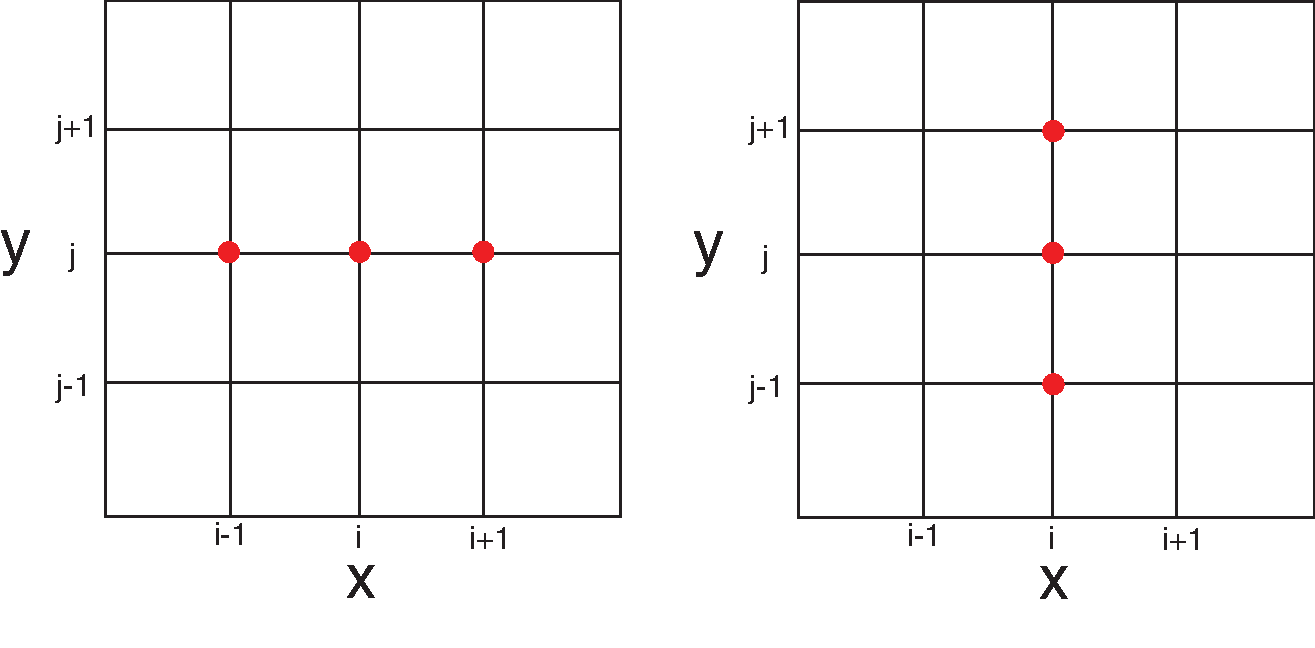
\includegraphics[width=0.7\textwidth]{grid_x.pdf} 
\caption{ Finite differences in the $x$ and $y$  directions for a two dimensional grid. }
\label{grid}
\end{center}
\end{figure}

Inserting these into Laplace's equation gives:
\begin{eqnarray}
	     \frac{u_{i+1,j} - 2 u_{i,j}+ u_{i-1,j}  }{\Delta x^2}  +  \frac{u_{i,j+1} - 2 u_{i,j} + u_{i,j-1}  }{\Delta y^2}   = 0.
\end{eqnarray}
If we assume our grid spacing is even in the $x$ and $y$ directions so $\Delta x = \Delta y$, we can factor out the $\Delta x$ and $\Delta y$ terms. Rearranging the resulting expression  for $u_i$ yields:
\begin{eqnarray}
	 u_{i,j}    =  \frac{1}{4} \left ( u_{i+1,j}  + u_{i-1,j}  + u_{i,j+1}   + u_{i,j-1} \right )    
\end{eqnarray}
Here you can see that the central value $u_{i,j}$ is simply the average of all its neighbors!  See Figure \ref{gridlaplace}.

In class we will go over how to write an iterative loop that solves Laplace's equation using this averaging equation.
 
\begin{figure}[htbp]
\begin{center}
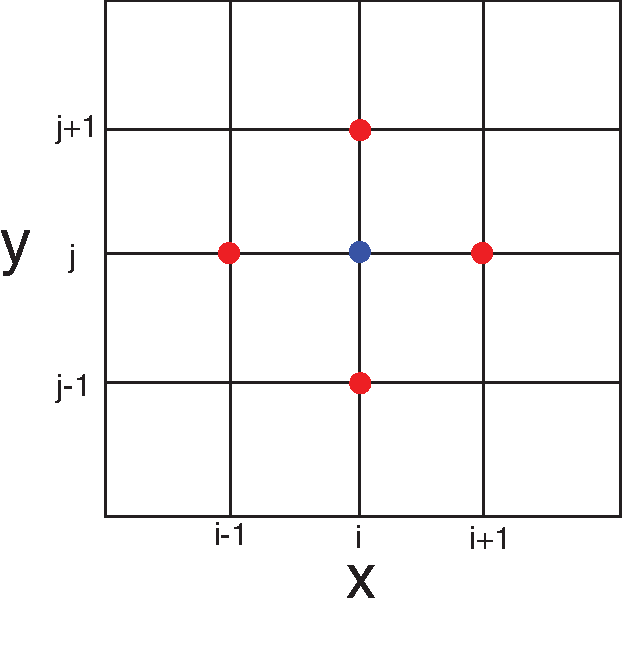
\includegraphics[width=0.5\textwidth]{grid_laplace.pdf} 
\caption{ Finite difference stencil for Laplace's equation at point $x_i,y_j$. }
\label{gridlaplace}
\end{center}
\end{figure}


 
\end{document}  